% Hopefully this will be the final version of Problem statement.
In this chapter, we present an introduction to the problem that will be addressed in this thesis. 

\section{Problem Statement}

% \bx{What is Cloud computing and why it is the pillar of software and other related industry. (Importance of Cloud computing.)}
% \bx{
% \begin{itemize}
% 	\item (What) The main challenge for Cloud provider is to reduce energy consumption
% 	\item WHY it is important and SO WHAT? (consequences?),
% 	\item HOW to deal with it? (Technologies)
% \end{itemize}}
\bx{Cloud computing is a major shift on modern software industry by offering on-demand computing capacity (e.g storage and  computing) over the Internet \cite{2010arXiv1006.0308B}}. With no upfront investment, low price, and high availability (e.g services are accessible 99.99\% of the time), most web service providers such as Google and Neflix tend to deploy their services (e.g. Google drive) on Cloud. 

\bx{A major issue in Cloud computing is the huge energy consumption generated by data centers} - a typical data center consumes as much energy as 25,000 households \cite{Dayarathna:2016ua}. Since energy has become the major expense of cloud providers, cutting the energy bill becomes a critical mission which will lead to a cost reduction of software and consequently be beneficial to most people who access the Internet on a daily basis.

\bx{To reduce the energy consumption of a data center, the main target is to reduce the usage of physical machines (PMs) (e.g. servers).} In a data center such as cooling system, PMs, and network devices, PMs accounts for the majority - more than 40\% - of energy consumption.Therefore, it is possible to reduce energy by improving the utilization of PMs. Currently, because the defects in resource management, PMs always run in a low utilization \cite{Barroso:2007jt, Shen:2015hm} - from 10\% to 50\% of required resources on average.
% This is because cloud users tend to preserve more resources in order to guarantee the performance when facing the variation of workloads.



\bx{The major way to reduce the energy consumption of PMs is through resource management \cite{Manvi:2014hm} (see Figure \ref{fig:workflow}).} Generally, cloud resource management is a centralized system \cite{Jennings:2015ht} that allocates resources to cloud users' applications, handles the workload fluctuations. Better management of application placement and workloads leads to the reduction of PMs and energy. 

\bx{One of the crucial steps in resource management that related to energy consumption is \emph{placement decision}}. Placement decision determines the location of applications based on the resource requirement provided by data analysis. The decision involves with an optimization process called server consolidation which decides the placement of applications for the best energy efficiency. 
\begin{figure}
	\centering
	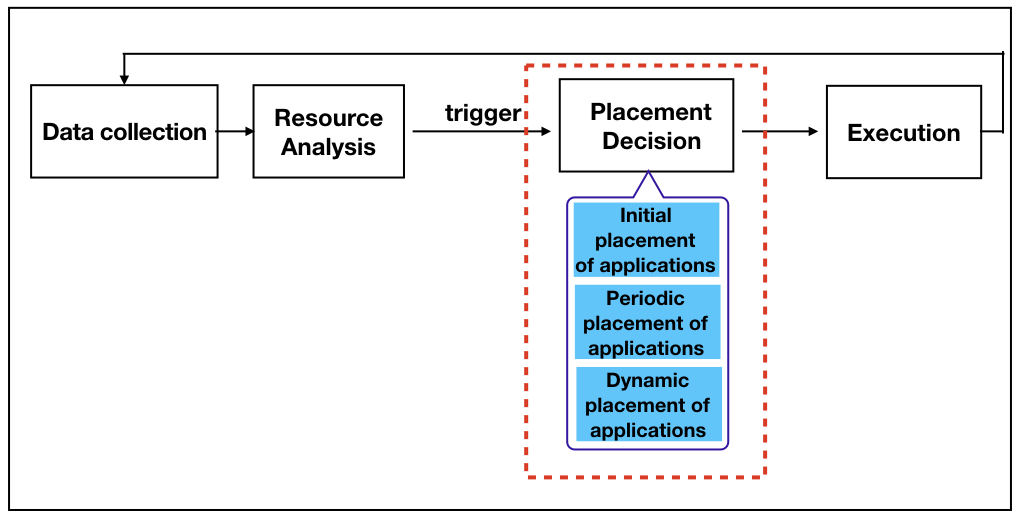
\includegraphics[width=0.7\textwidth]{pics/workflow_management.png}
	\caption{A workflow of resource management \cite{Mishra:2012kx}}
	\label{fig:workflow}
\end{figure}

% Data collection gathers resource utilization information from individual PMs and VMs such as CPU, memory utilization in a period of time. These data are collected by monitoring softwares for data analysis. Data analysis takes the collected data as the input, cleans and analyzes them. It outputs the quantity of demand resources of applications. Finally, execution places the applications to the target PMs. 

% \bx{Among these resource management steps, placement decision is the crucial step which includes three scenarios: application initial placement, periodic optimization and overloading & under-loading adjustment.} Essentially, these three scenarios contain a common strategy called server consolidation.

\bx{Server consolidation \cite{Varasteh:2015fu} is an approach to efficiently use the resources of PMs in order to reduce the total number of PMs which leads to lower energy consumption.} For three resource management scenarios, server consolidation is applied in different ways: static and dynamic. Static approach is conducted in an off-line fashion: application initial placement and periodic optimization belong to this category, while dynamic approach is conducted in an on-line fashion: over-loading and under-loading scenarios are in this category.


\bx{Currently, resource management in data centers is based on \emph{virtualization} technology\cite{Uhlig:2005do}. } Such virtualization separates the resources (e.g. CPUs and RAMs) of a PM into several parts called \emph{virtual machines (VMs)}, each of which runs an isolated operating system. Before virtualization technology was widely used, traditional data center assigns a PM for each application; it leads to the low utilization of PMs. Later on, by using VMs to deploy applications, the utilization of PMs has been largely improved and energy consumption are reduced. 

\bx{However, in recent years, resource management with VMs cannot catch up with a new trend in software industry - Service Oriented Architecture (SOA) \cite{Sprott:2004wt};} SOA has become widely used in modern software industry because of its agility and re-usability \cite{Sprott:2004wt}. SOA separates a centralized application into multiple distributed components called web services. As most of web services only require a small amount of resources,  using a VM for a web service causes resource wastage inside a VM. Consequently the low utilization of PMs decreases the energy efficiency. 


\bx{To resolve the wastage of resource and energy in SOA by using VMs, a new virtualization technology: containers \cite{Felter:2015ki, Soltesz:2007cu} and a new service model: Container as a Service (CaaS) \cite{Piraghaj:2015uf} have been proposed to provide a finer granularity level of resource management.} Container is an operating system (OS) level of virtualization which run on top of VMs. A container provides performance and resource isolation for a single application so that multiple applications can run in the same VM without interfering each other. In addition, containers naturally support vertical scaling (change its size during runtime)\cite{Vaquero:2011gb} which is resilient to the fluctuate workloads.  CaaS uses containers as the fundamental resource management units. Thus, CaaS has the potential to improve the utilization of resources as well as energy consumption \cite{Esposito:2016br}. 







Container is still a young technology which brings new challenges in server consolidation. We will discuss these challenges in terms of three placement decision scenarios: application initial placement, periodic optimization, and dynamic placement.

% \bx{Despite which virtualization is used, server consolidation can be applied in three resource management scenarios:} application initial placement  \cite{Jennings:2015ht}, periodic optimization \cite{Mishra:2012kx} and overloading/under-loading adjustments \cite{Mishra:2012kx} (see Figure \ref{fig:workflow}).

 % Server consumption is essentially an optimization task where it adjusts applications' locations in PMs so that a minimum number of PMs is used. For a certain number of applications, the fewer number of PMs is used, the less energy is consumed. 

% Three management processes: application initial placement, periodic optimization ,   have distinct characteristics, hence, the server consolidation techniques applied on them can be roughly classified into two categories: static \cite{Xiao:2015ik} and dynamic \cite{Beloglazov:2012bw}.

% \bx{In Initial application placement, the consolidation can be described as a static task conducted in an off-line manner.} 
\vspace{5mm}
